\problemname{Qanat}

A {\em qanat\/} is an irrigation system widely used to deliver water in
hot, arid climates. The technology was originally developed by Persians
over 2000 years ago. In Morocco, qanats are known as khettara and are 
still used today in the southern part of the country.

The basic feature of a qanat is an essentially horizontal channel that
brings water from an underground water source to an outlet near a
civilization. There is also a shaft known as a {\em mother
well\/} that rises vertically from the underground water source to the
surface of a mountain or hill. Creating such a system is extremely
expensive, and was especially so in ancient times, since all of the materials
excavated from the channel and mother well must be carried above ground,
either through the channel outlet or the top of the mother well.
To aid in the construction, there are often one or more additional
vertical shafts placed at strategic locations above the underground
channel. Although these shafts must also be excavated, they provide
a means for lifting additional dirt from the horizontal channel as illustrated in Figure \ref{fig:qanat}.

\begin{figure}[!h]
\centering
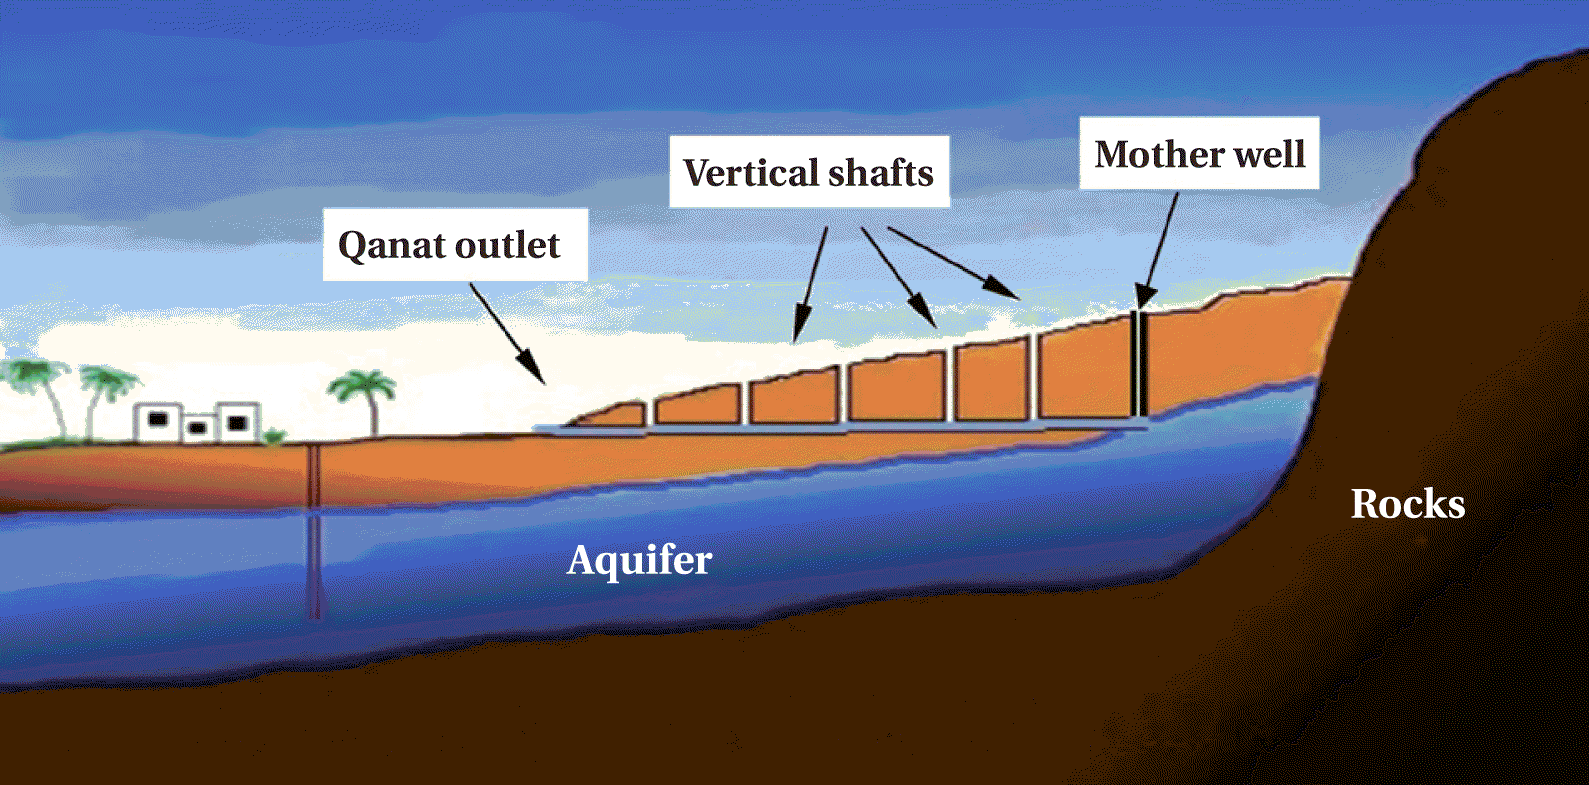
\includegraphics[width=0.55\textwidth]{qanat}
\vspace{-0.5cm}
\caption{An illustration of a qanat.}
\label{fig:qanat}
\end{figure}

For this problem, model the cross-section of a qanat as shown in
Figure~\ref{fig:model}, with the channel outlet at $(0,0)$,
the water source at $(w,0)$, and the top of the mother well at $(w,h)$ with $w > h$. The
surface of the mountain extends along a straight line from $(w,h)$ to $(0,0)$.

\begin{figure}[!h]
\centering
\includegraphics[width=0.5\textwidth]{triangle}
\caption{A simplified model of a qanat cross-section.}
\label{fig:model}
\end{figure}

Every qanat must have a vertical mother well from the water source to
the mountain surface above, along with $n$
additional vertical shafts. The channel and all shafts are modeled as
line segments. Your goal is to determine the placement
for those additional shafts so as to minimize the overall
excavation cost. This cost is equal to the sum of the
distances that each piece of excavated dirt  must be transported to reach 
the surface (using any combination of horizontal and vertical
movement). For example, the cost of excavating a continuous section of
dirt starting from the surface and going along a path of length~$\ell$ (possibly including
turns) is $\int_0^{\ell} x \,dx = \frac{1}{2} \ell^2$.

\section*{Input}
The input consists of a single line containing three integers $w$
($1 \le w \le 10\,000$), $h$ ($1 \le h < w$), and $n$~($1 \le n \le
1\,000$). The value $w$ is the horizontal distance from the water
source to the qanat outlet. The value $h$ is the vertical distance
from the water source to the mountain surface. The value $n$ is the
number of vertical shafts that must be used in addition to the mother
well.

\section*{Output}
First, display the minimum overall excavation cost.
Next, display the $x$-coordinates, in increasing order, for
$n$ optimally placed vertical shafts.  If $n > 10$, display only the first $10$ $x$-coordinates.
Answers within an absolute or relative error of $10^{-4}$ will be 
accepted.  You may assume that there is a unique solution.
No test case will result in a shaft within $0.001$ 
units from the outlet of the qanat channel or from another shaft.
